\section{Results}

The methodology we present uses data on land use and block size extracted from maps and deploys a Self Organising Map (SOM) algorithm to organise them. SOM is an unsupervised sorting algorithm that iteratively sorts a list of vectors (containing higher dimensional information), projecting them into lower dimensions, adding a spatial component by moving similar vectors closer and spreading dissimilar vectors further away.

We demonstrate the method using information derived from 300$\times$300m map segments of 1.7 million locations sampled from the world's largest cities (populations greater than 300,000). The results are a 2-dimensional map of clusters of neighbourhood types seen in the 1667 cities where 2.2 billion people currently live. Figure \ref{fig:somresults} shows a visualisation of the results of this process. Each (x,y) node location in the SOM can contain either zero maps (and is shown in black) or a single or many maps (and is represented by one of the maps). A colour scheme map (Figure \ref{fig:colormap}) is used to convert the (x,y) locations into red/green/blue (RGB) values to plot the spatial distributions of neighbourhood types in Tokyo and New York, for example, see Figures \ref{fig:citylocations}a and \ref{fig:citylocations}b. Visualisations of the SOM showing only locations in Tokyo and New York are shown in Figures \ref{fig:citylocations}c and \ref{fig:citylocations}d. Red Boxes and Lines (i, ii, iii, and iv) in Figure \ref{fig:citylocations} connects some example spatial regions in these cities to their corresponding neighbourhood types.

\begin{figure}
\centering
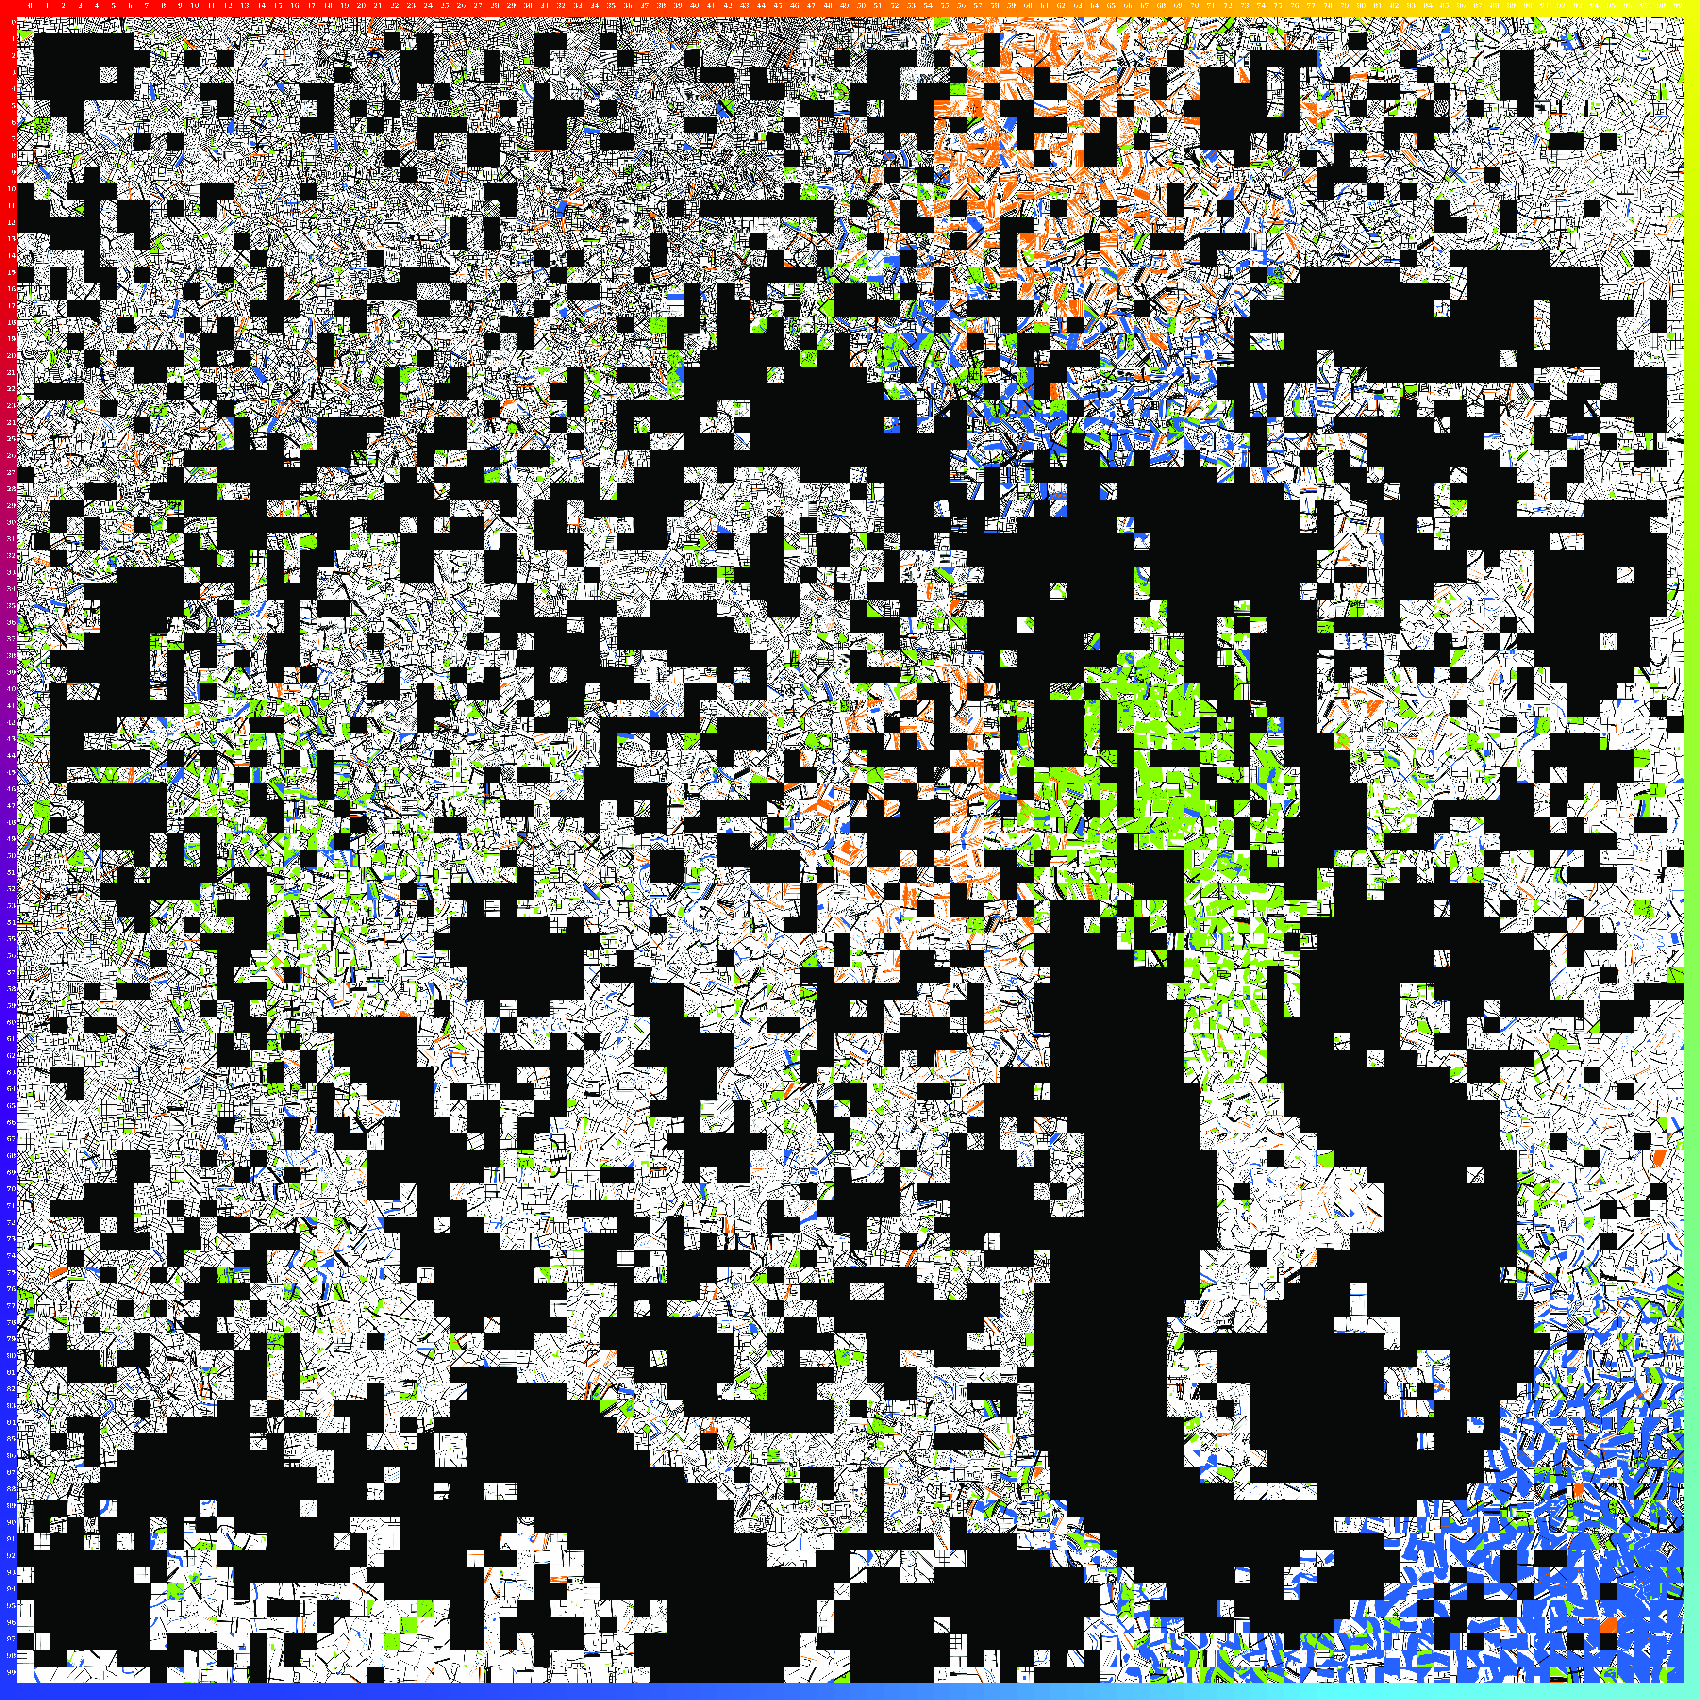
\includegraphics[trim={0 0 0 0},clip,scale=0.17]{BlockTypologies_Figures2-0.png}
\caption{\bf A visualisation of the 2-dimensional 100$\times$100 SOM trained with 1.7 million map images from 1667 cities. Each (x,y) point shows a representative image associated with each node while nodes without associated images are shown in black. Border shows colour coding scheme (Figure \ref{fig:colormap}) for SOM (x,y) locations used in Figure \ref{fig:citylocations}.}
 \label{fig:somresults}
\end{figure} 

\begin{figure}
\centering

\includegraphics[trim={0 0 0 0},clip,scale=0.15]{cubediagonal.png}
\caption{\bf Colour map used to plot SOM (x,y) locations in Figure \ref{fig:citylocations}. }
 \label{fig:colormap}
\end{figure} 

\begin{figure}
\centering
%\frame{
%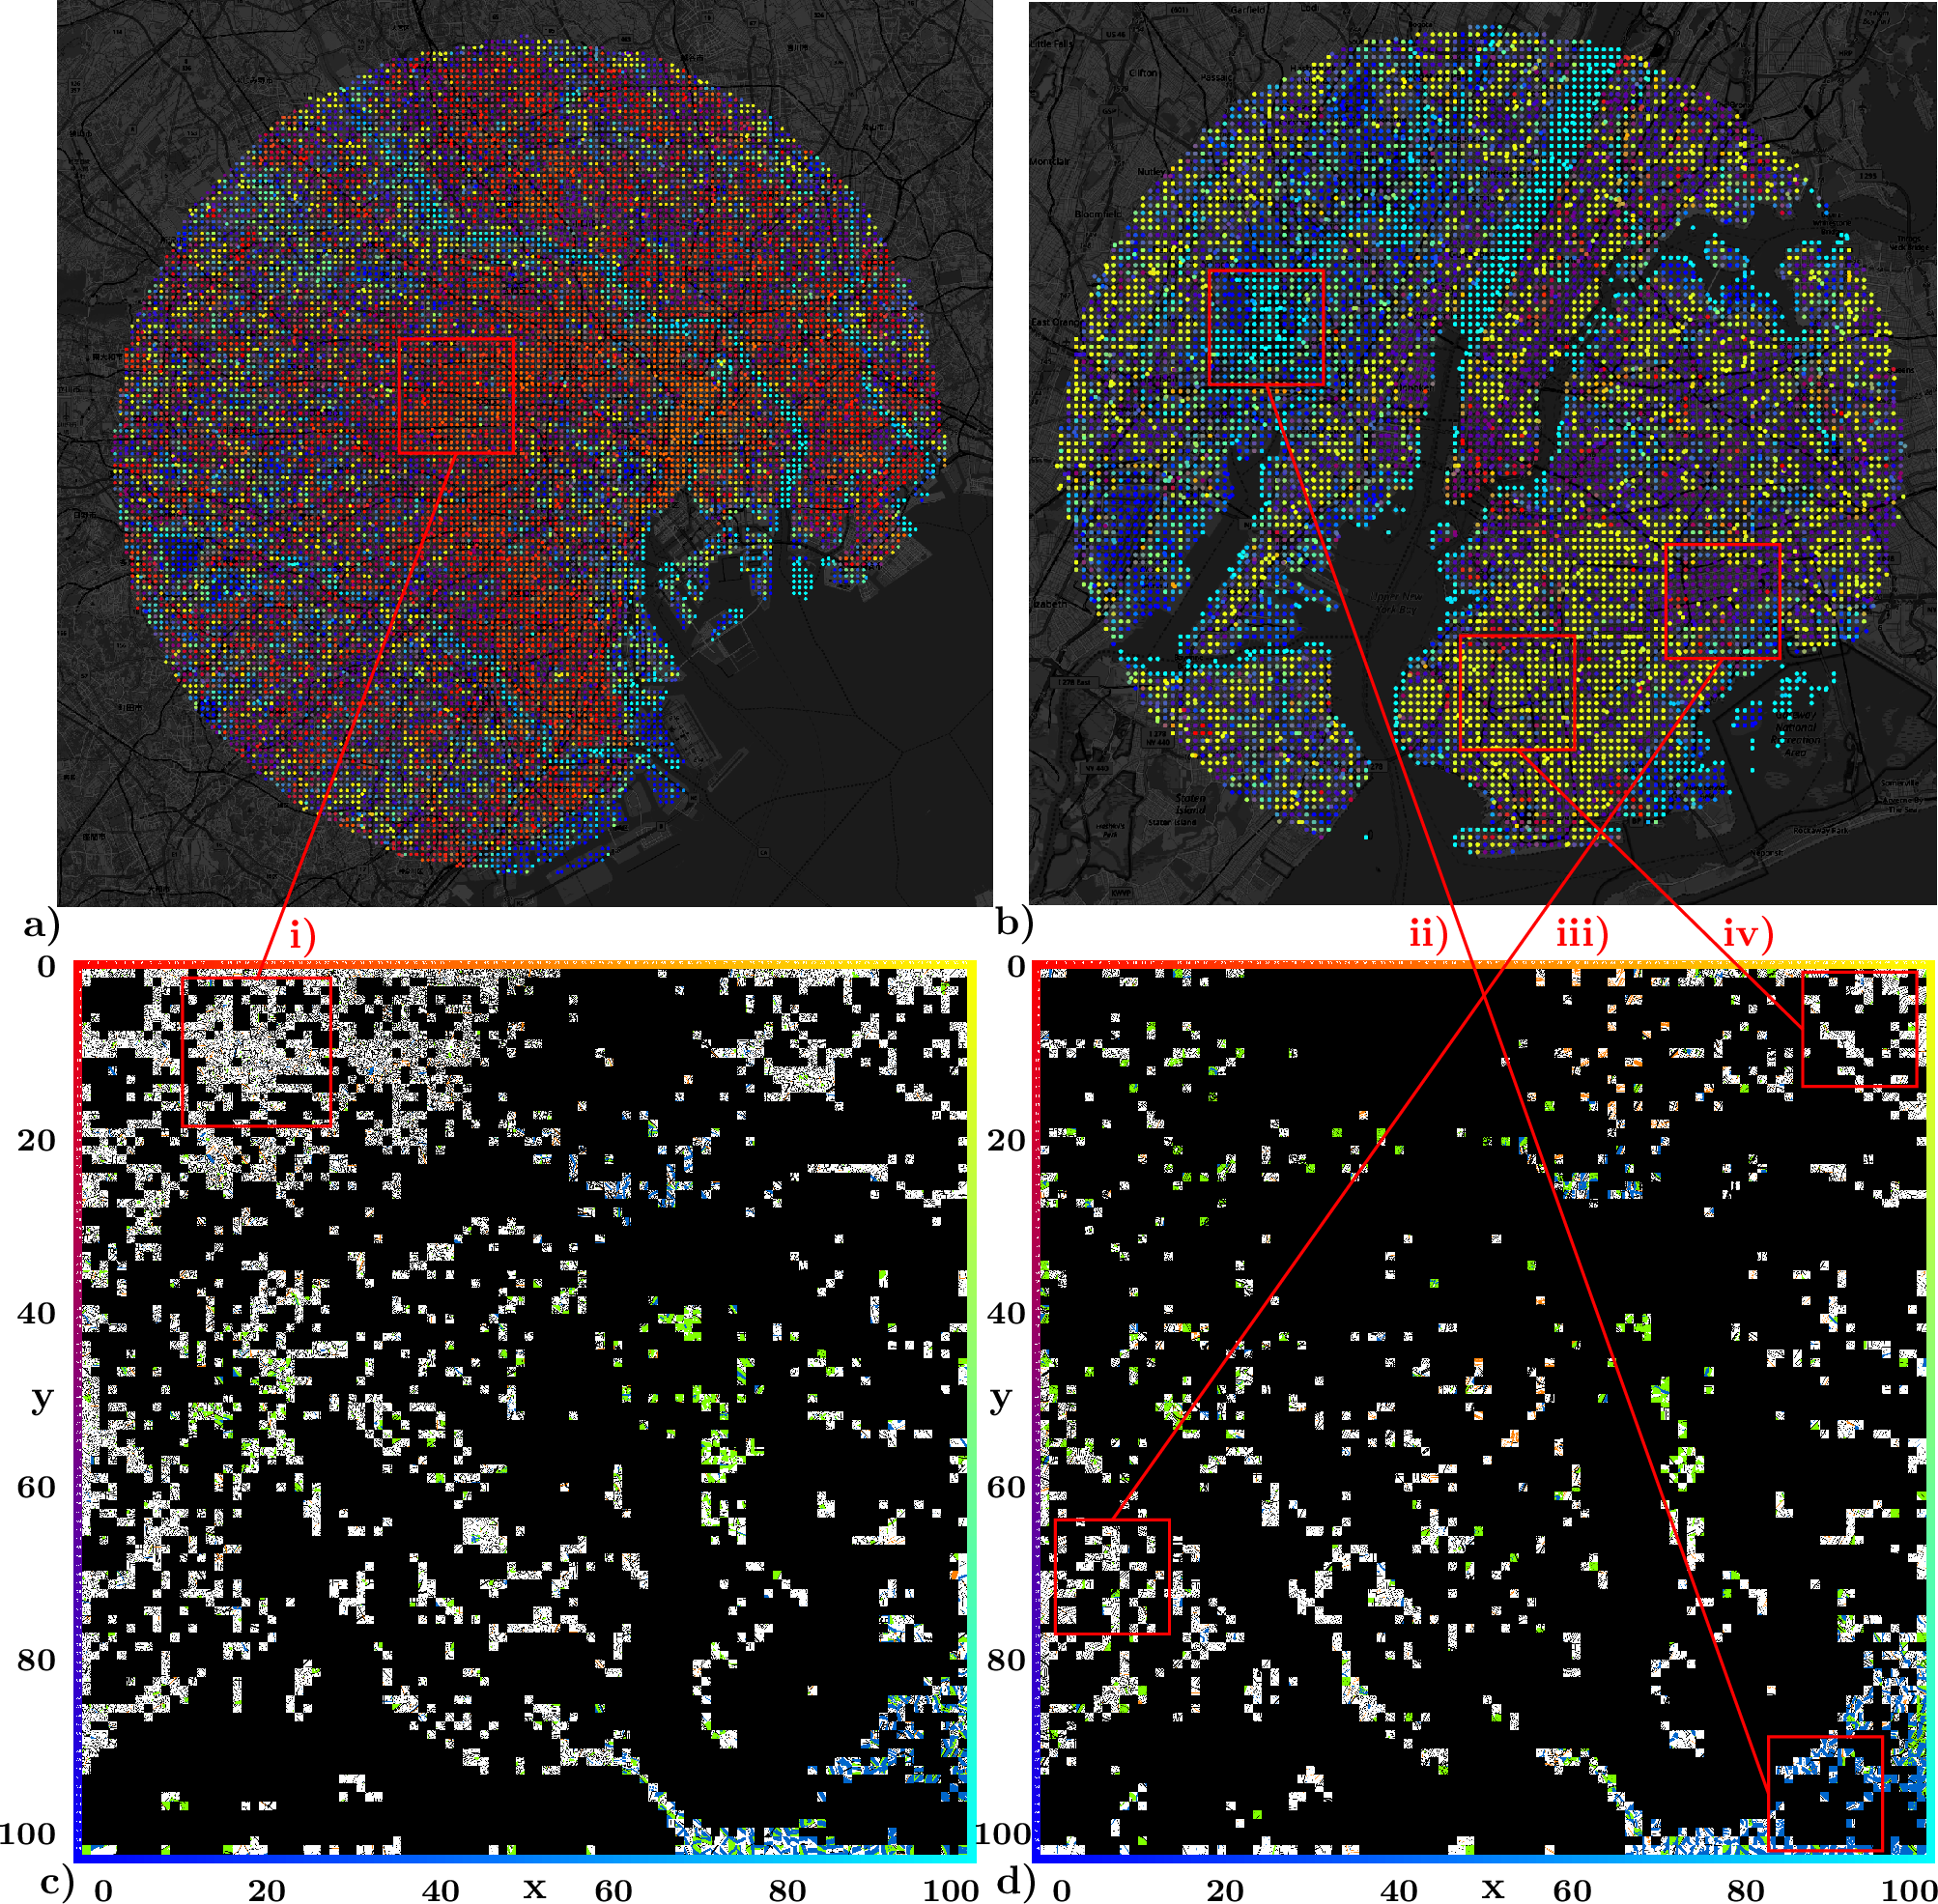
\includegraphics[page=1,trim={58 180 54 188},clip,scale=0.95]{BlockTypologies_Figures5.pdf} 
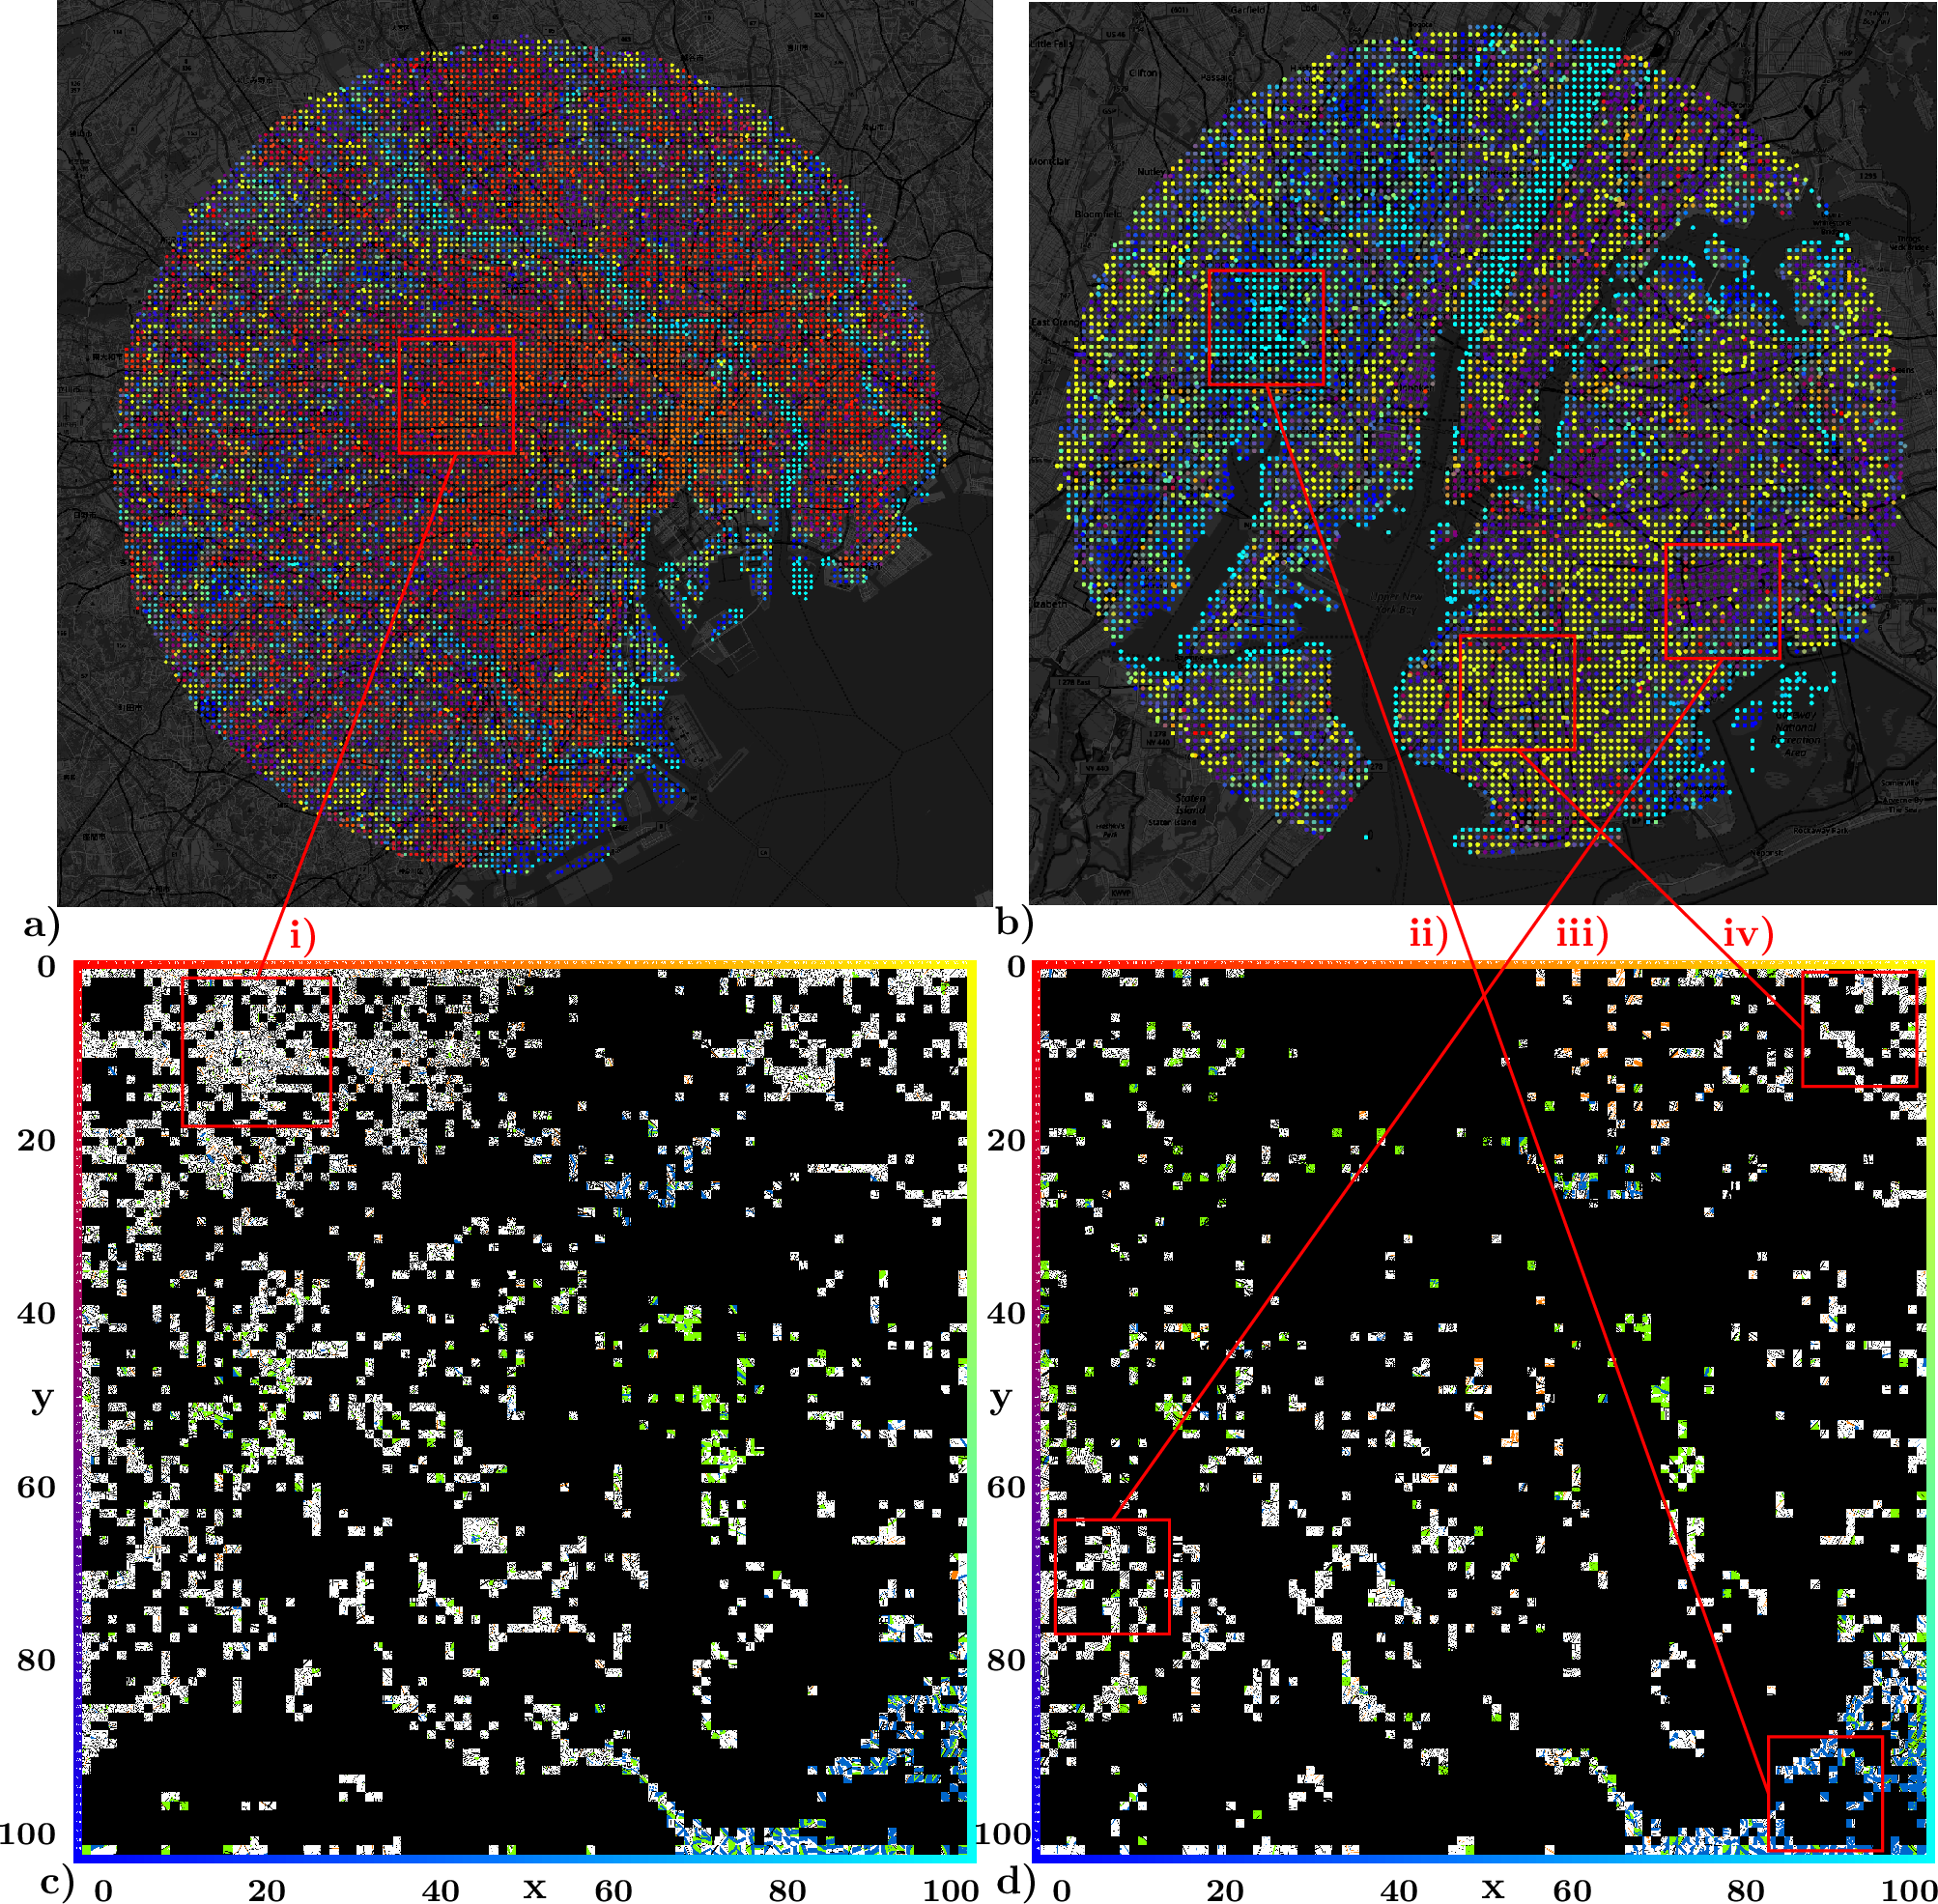
\includegraphics[trim={0 0 0 0},clip,scale=0.23]{BlockTypologies_Figures5.png} 
% }
\caption{\bf Spatial distribution of neighbourhood types (as represented by SOM (x,y) locations) in a) Tokyo and b) New York. City detail maps use the same SOM (x,y) location colour scheme as the border of Figure \ref{fig:somresults} and of Figure \ref{fig:colormap} colour map. SOM visualisation of Figure \ref{fig:somresults} but only displaying locations in c) Tokyo and d) New York. Red boxes and lines i, ii, iii, and iv show neighbourhood types (bottom) corresponding to locations (top) within Tokyo and New York.}
 \label{fig:citylocations}
\end{figure} 

Using these figures, it can be seen that in Tokyo, neighbourhoods of very small irregular blocks, depicted by the (10,15) orange type (Figure \ref{fig:citylocations} Line i), are concentrated within the inner ring road. In the waterfront areas, a mix of of larger and less structured blocks and mixes of water and green space correspond to the blue and aqua types (SOM areas below the 60 y-axis). The eastern part of the city continues with predominately small irregular blocks while the western side shows a more heterogeneous mix. 

In New York, Brooklyn is predominately large regular gridded blocks (Figure \ref{fig:citylocations} Line iv) depicted by the (98,8) yellow-green types. Queens is a mix of yellow-green types, mixed sized slightly irregular blocks (Figure \ref{fig:citylocations} Line iii) corresponding to (10,70) purple types, and mixed water/green and large blocks (Figure \ref{fig:citylocations} Line ii) of the (85,98) blue type. Purples continue into lower and mid-Manhattan, transforming into a mix similar to Brooklyn in uptown Manhattan and the Bronx. A strip of yellow-green runs north-south down east New Jersey with blue and purple fringes on the water edges.

To validate the application, we calculated mean averages for each (x,y) location (using the 1000 nearest neighbours) in the SOM and the latitude/longitude of those locations using a number of gridded observational datasets of pollution and emissions. We also used a dataset of fractions of classes of urban form, including trees, impervious surfaces, and non-permanent objects (i.e. moving vehicles) calculated from Google Street View at 65 million locations in 70 cities\cite{Middel2019,Middel2018}. Both these datasets enable a validation that block size and regularity can be used to find neighbourhood types reflecting their actual morphology, but also provide insights into how these morphologies reflect transportation infrastructure decisions (allocated road space, amounts of vehicles, and population density) and the impacts of those choices (emissions and air pollution). Figure \ref{fig:meansomresults} shows mean values for the SOM of percentage of a) tree cover and b) impervious surfaces, as well as levels of c) NO$_{2}$, d) population density (from SEDAC dataset), e) Aerosol Optical Depth (AOD), and f) fossil fuel CO$_{2}$ emissions intensity (from FFDAS dataset).

\begin{figure}
\centering
%\includegraphics[page=1,trim={65 295 65 295},clip]{../Article-BlockTypologies/BlockTypologies_Figures4.pdf}
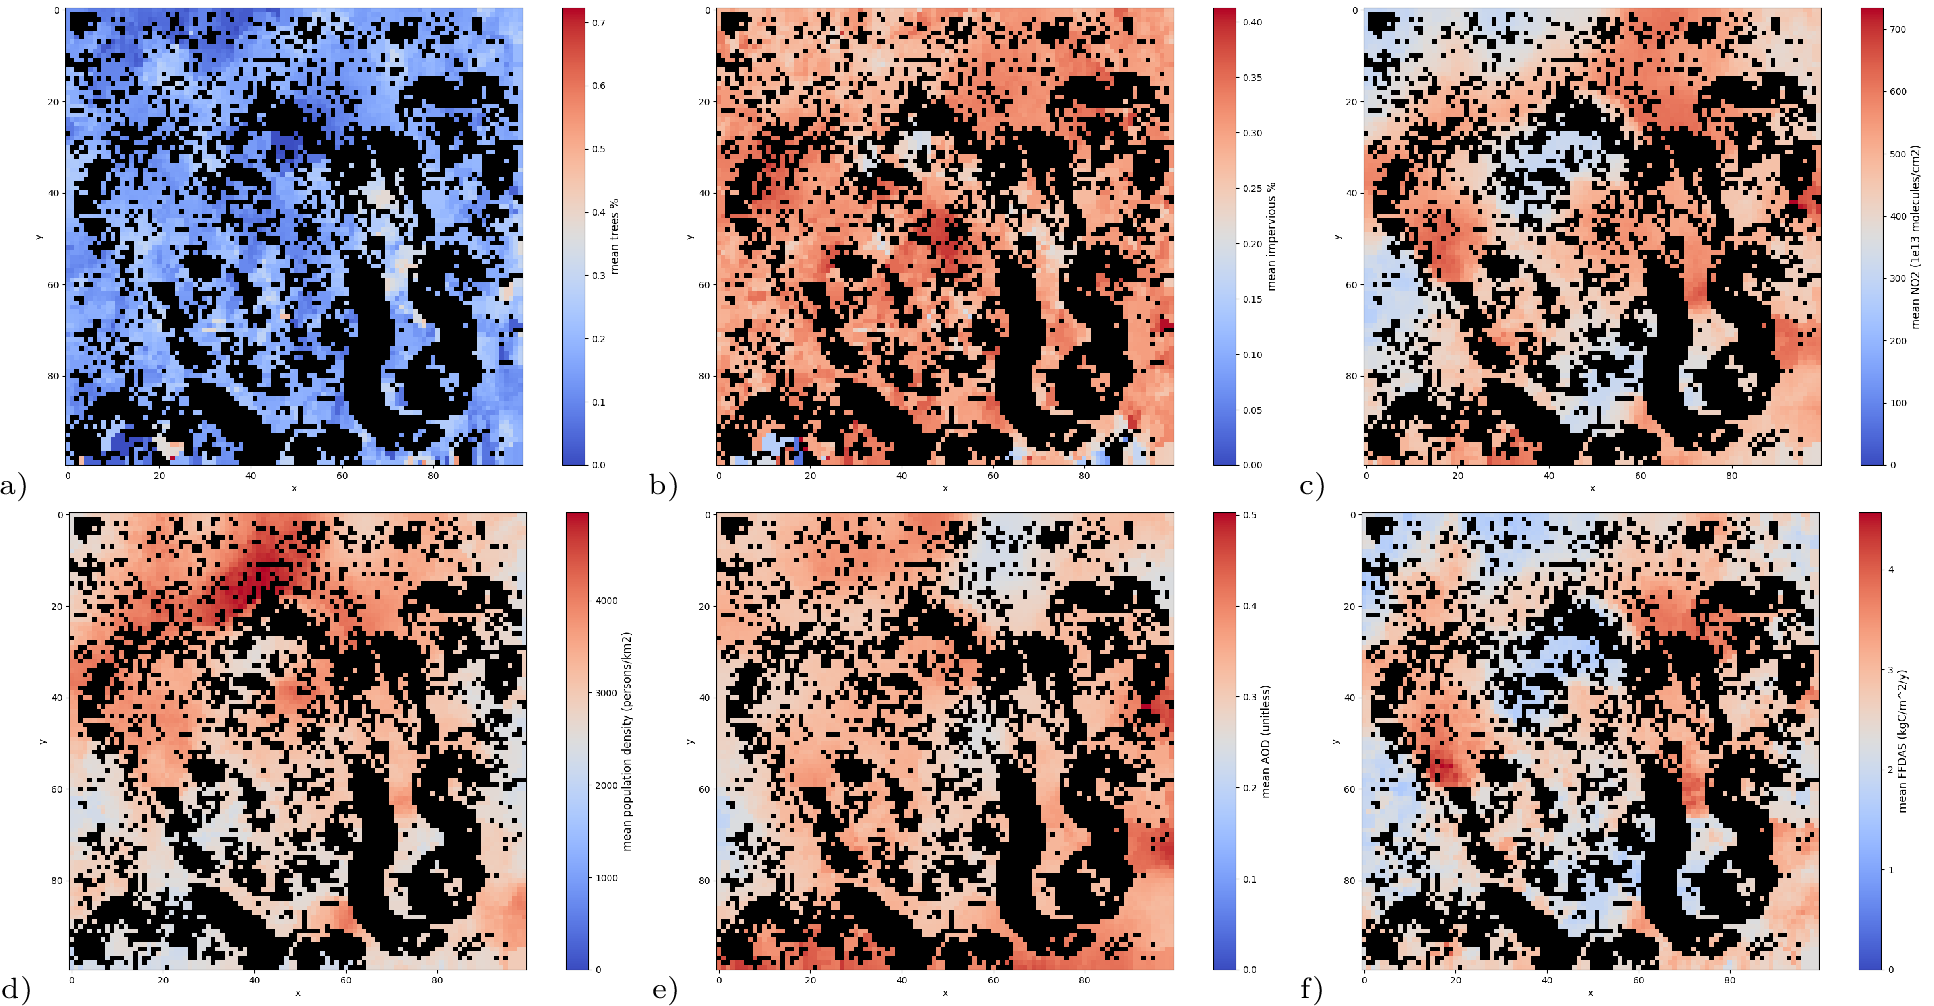
\includegraphics[trim={0 0 0 0},clip,scale=0.23]{BlockTypologies_Figures4-0.png}
\caption{\bf Mean averages for each SOM (x,y) location from Figure \ref{fig:somresults} using the 1000 nearest neighbours. Means calculated using observed values of fractions of a) trees and b) impervious surfaces and values of c) NO$_{2}$, d) population density, e) Aerosol Optical Depth (AOD), and f) fossil fuel CO$_{2}$ emissions intensity (FFDAS).}
 \label{fig:meansomresults}
\end{figure} 

It can be observed in Figure \ref{fig:meansomresults}a, that higher fractions of tree cover correspond to regions in Figure \ref{fig:somresults} with high levels of green space, including (65,40), (22,95), (75,60), and (95,60). In Figure \ref{fig:meansomresults}b, small amounts of impervious surfaces are observed at 95 on the y axis where the map segments show low density streets and areas of high blue space. For population density, Figure \ref{fig:meansomresults}d shows high population density across the (40,20) region where the SOM shows extremely dense street networks and reductions in density moving down the y axis from 60 to 100 where the SOM shows very low density less structured street networks.

While the previous examples (tree cover, surface types, and density) show relationships that can be easily derived from direct observations of urban areas, Figures \ref{fig:meansomresults}c, e, and f show relationships between pollution and urban form that are not possible to observe directly. There are very similar responses to urban form types between NO$_{2}$ and carbon intensity (FFDAS). Areas with high values around (99,40), (20,58), (68,60), and (66,25) correspond to areas with large (often regular) blocks, often combined with a light mix green and blue space. Areas with low values are seen around (45,30), (10,10), (30,5), areas with a very dense mix of and intricate street network and (5,60) and (50,90), areas of slightly less dense street structure. However, AOD often shows a different relationship with urban form than NO$_{2}$ and FFDAS. Where regions around (5,60) show reduced levels of AOD (similar but to a lesser extent to NO$_{2}$ and FFDAS), the areas around (45,30), (10,10), and (30,5) show higher levels of AOD (the inverse of NO$_{2}$ and FFDAS). 

As a further validation, we calculated correlations between mean average values of pollution and elements of urban form for each city compared to averages of weighted averages of the mix of SOM(x,y) locations for each city (Table \ref{table:correlations}). Good correlations are observed for fractions of urban form (ranging from 0.97 to 0.56) as well as good correlations (ranging from 0.58 to 0.57) with pollution levels. Again, these results provide insights into the urban morphological make-up of different cities and transportation decisions underlying each neighbourhood type and the impacts of those choices.

\begin{table}
\centering
\caption{Correlations between mean average values by city and by (x,y) location within the SOM.}\label{table:correlations}
\begin{tabular}{ | c | c |}
\hline \textbf{Parameter} & \textbf{Correlation value}\\ \hline
Movable objects fraction& 0.97 \\ \hline
Impervious surfaces fraction& 0.86 \\ \hline
Sky fraction& 0.75 \\ \hline
Building fraction& 0.56 \\ \hline
Mean AOD& 0.58 \\ \hline
Mean NO$_{2}$&0.57 \\ \hline
\end{tabular}
\end{table}



\section{Broader Implications}

A look at the range of neighbourhood typologies from individual cities shows that many cities are an eclectic mixture of different neighbourhood typologies but all are built using common elements. An individual city's uniqueness (in this case, the city's structure through its blocks and streets), what we refer to as the city's `fingerprint', is reflected in an individual mix of neighbourhood typologies, with Figure \ref{fig:kernel} showing a number of city `fingerprints' based on the concentration of neighbourhood types. These individual fingerprints can be used to compare cities around the world at a granularity of individual 300$\times$300m neighbourhoods. We find that the uniqueness of cities are derived from a subtle mix of common elements and their spatial distribution (Figure \ref{fig:citylocations}).

\begin{figure}
\centering
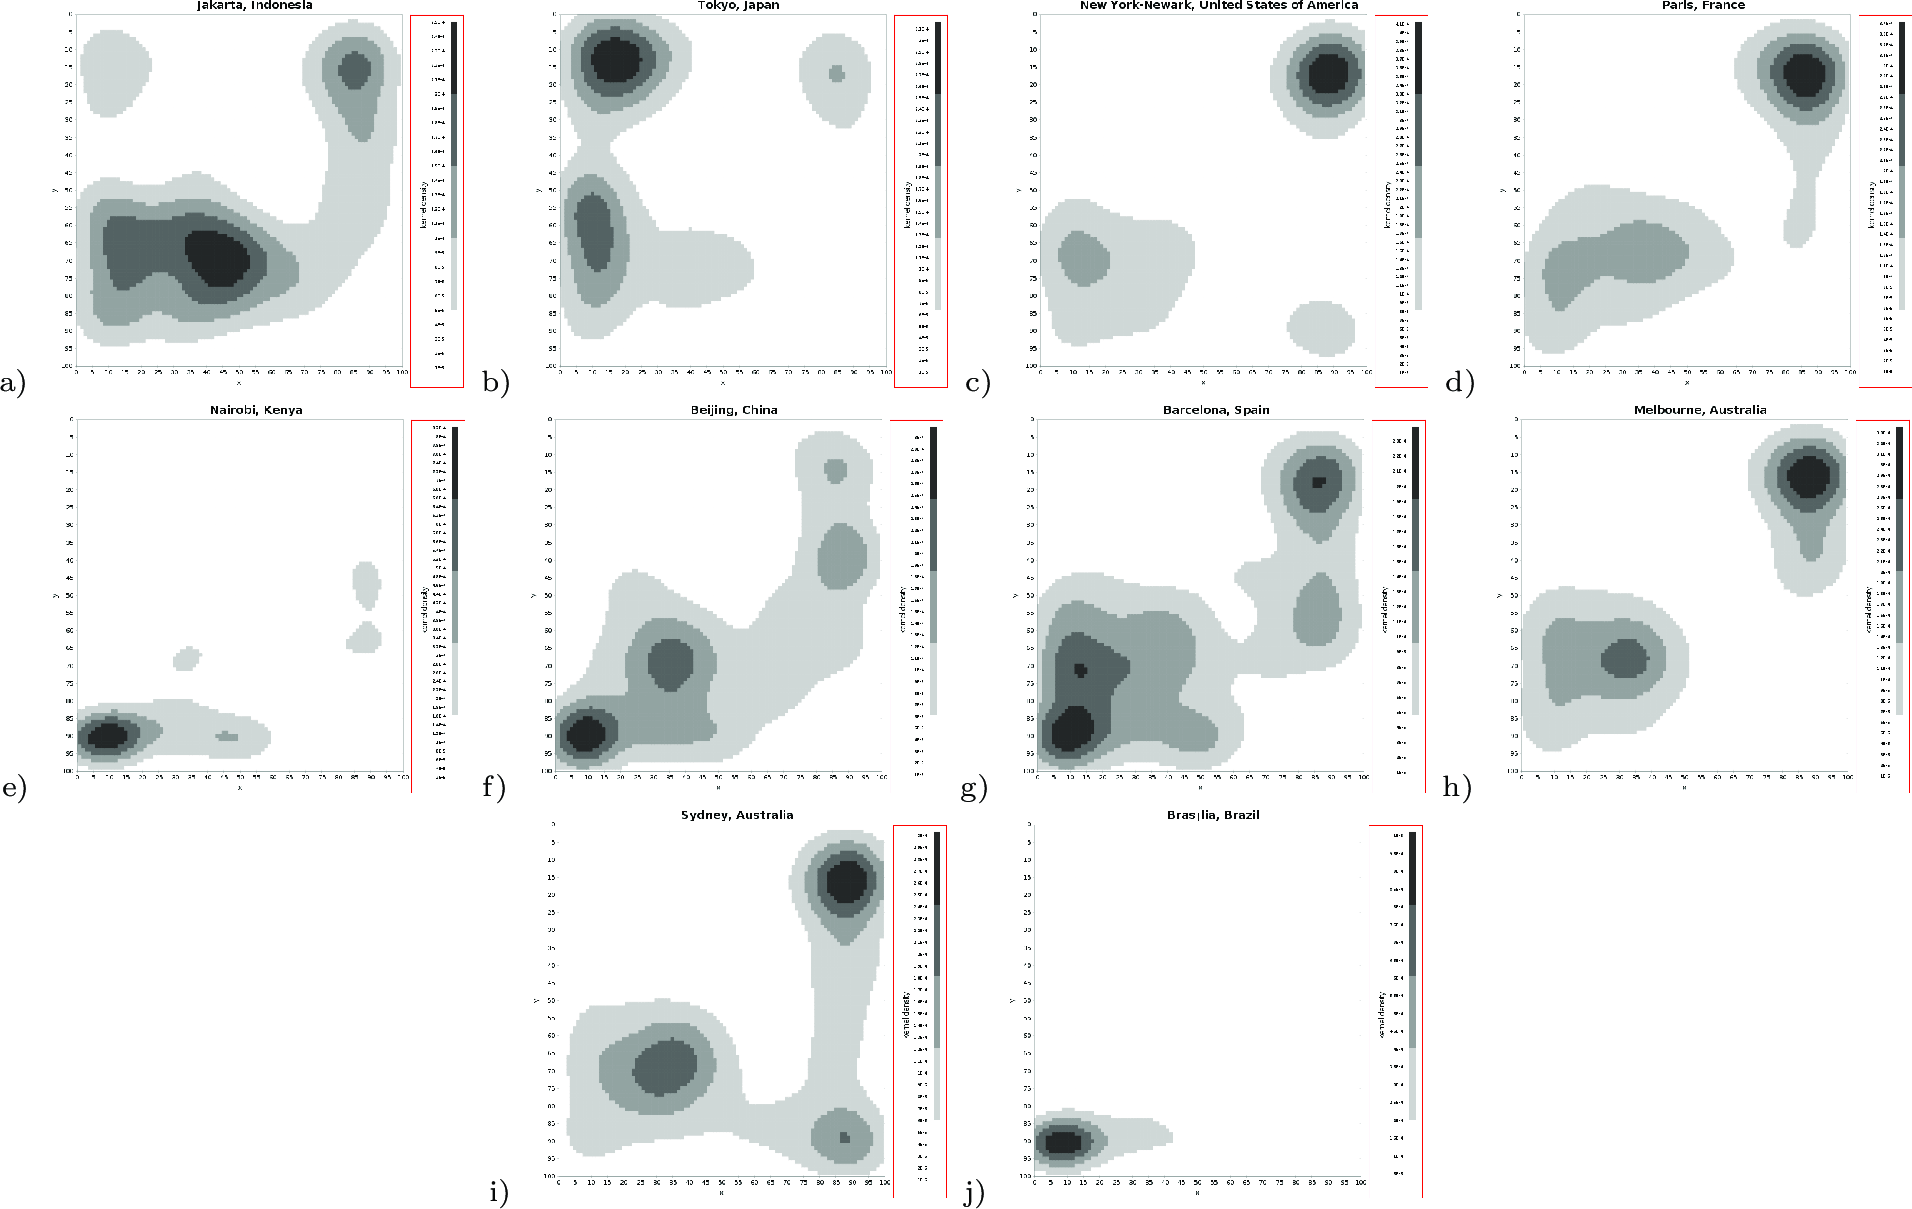
\includegraphics[trim={0 0 0 0},clip,scale=0.17]{BlockTypologies_Figures2-1.png}
\caption{\bf City fingerprints generated by kernel density maps of SOM (x,y) locations for cities 
a) Jakarta,
b) Tokyo, 
c) New York, 
d) Paris,
e) Nairobi,
f) Beijing, 
g) Barcelona, 
h) Melbourne, 
i) Sydney, and
j) Bras\'{i}lia.
}
 \label{fig:kernel}
\end{figure} 

This provides insights at an unprecedented granularity, uncovering the mix and scale of neighbourhoods across these cities. We have found unique individual neighbourhood types that can have twins in different cities across the globe. We also show the extent to which individual cities are heterogeneous within their bounds and the variation in distribution of neighbourhood types they display. Finally, we show associations between the mixes of neighbourhood typologies derived through our method to both the amounts of different amounts of urban form and the contribution of these neighbourhood typology mixes to measured levels of pollution (as one measure of their performance) in each city. 

Our unique contribution is a method that allows, for the first time, global inter-comparisons of neighbourhoods while highlighting that cities are constructed using fundamental particles; neighbourhood typologies. Due to the stability of the physical structure of cities, undergoing long term small incremental changes\cite{Wegener1986}, this collection represents a collective representation of the built history of human settlements. The implications are both fundamental and practical. It allows improvements to other systems such as health, transportation, and employment that are built on these fundamental components. The system can provide guidance for designers, engineers, stakeholders and policy makers by harnessing insights from a comparison across the globe. 

Our method has highlighted that cities are not unique and that individual neighbourhoods can be compared across continents. The findings also indicate that there is a common structure and that city typologies should be built across cities rather than within, that city centres are more comparable to other centres than to other elements of the same city. It also allows us now to compare cities on a global scale and investigate the nature of human settlements. The link between urban form and vehicle emissions has been shown on an aggregate level\cite{Frank2000}. Similarly, transportation mode choices are associated with block size and accessibility are a primary enabler/inhibitor for residence using active modes of transportation\cite{Ewing2001,Ewing2009a}. As shown in the results, we find strong correlations between different mixes of neighbourhood typologies derived through block size and regularity and the morphology and composition (through fractions of movable vehicles, sky view, buildings and impervious surfaces) of these areas. In addition, we find correlations between the mix of neighbourhood typologies and the performance of the city in terms of pollutants (AOD and NO$_{2}$). This method now allows us to investigate such questions at a neighbourhood scale. 

Finally, in contrast to previous methods which were limited by the available data from a handful of cities, this method is able to span the globe using available globally consistent map data. The method is also extendible and additional variables can be added to the vectors, such as demographic characteristics associated with each location\cite{Kropp1998}, distances to public transport, average building heights, or traffic counts to undercover extra dimensions of associations within the resulting neighbourhood typologies.



%       row    column       cor     p
%aodAquaObs     xyAodAqua     0.5833058 0
%aodTerraObs     xyAodTerra     0.5678217 0
%no2Obs      xyNo2         0.5714648 0 
%        SVFByCity          SVFByXY  0.695137382 7.142315e-06
% imperviousByCity   imperviousByXY  0.858961761 8.040502e-119
%     movingByCity       movingByXY  0.973403215 0.000000e+00
%   perviousByCity     perviousByXY  0.432223290 1.068619e-02
%        skyByCity          skyByXY  0.754313707 2.576413e-07
%      treesByCity        treesByXY  0.330958635 5.588998e-02 
% buildingByXY          0.5558685  1.000000e+00

